% TPM (DONE)
\section{TPM}
% ----------
\subsection{Chiffrements}
Une fonction de hachage $H$ prend une entrée $m$ de longueur variable et retourne un string de taille fixe $h$ (valeur hachée).
$$h=H(m)$$
\paragraph{Propriétés}
\begin{itemize}
    \item $H(m)$ est rapide à calculer
    \item $H$ est à sens unique
    \item $H$ est "collision-free"
\end{itemize}
% ----------
\subsubsection{Symétrique}
\begin{itemize}
    \item Même clé permet le chiffrement et déchiffrement
    \item Chiffrement par bloc, éventuellemnt chaîné (CBC - Cipher Block Chaining). IV (Initial Vector) non secret.
    \begin{figure}[H]
        \centering
        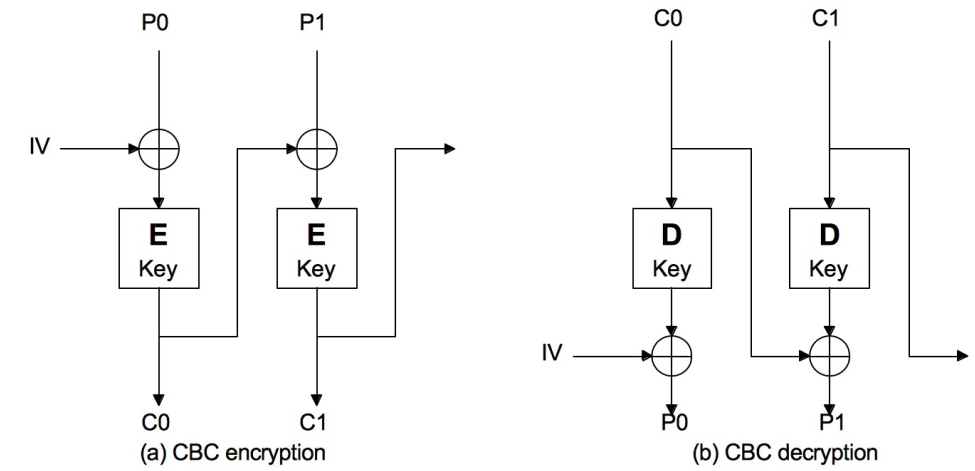
\includegraphics[width=0.75\columnwidth]{CBC.png}
    \end{figure}
\end{itemize}
% ----------
\subsubsection{Asymétrique}
\begin{itemize}
    \item Deux clés (publiques et privées) pour chaque partie, clé publique disponible par des certificats.
    \item Encrypt public $\rightarrow$ Decrypt private $\Rightarrow$ \textbf{confidentialité}, intégrité.
    \item Encrypt private $\rightarrow$ Decrypt public $\Rightarrow$ \textbf{authenticité} (signature numérique), intégrité.
\end{itemize}

\begin{figure}[H]
    \centering
    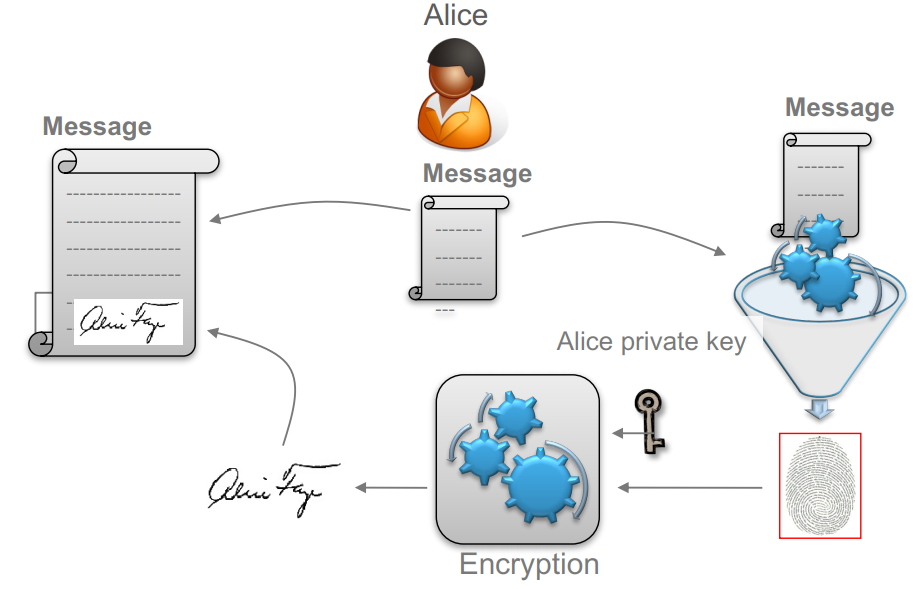
\includegraphics[width=\linewidth]{signature.png}
\end{figure}
% ----------
\subsection{TPM (Trusted Platform Module)}
$\Rightarrow$ coprocesseur cryptographique.
\begin{figure}[H]
    \centering
    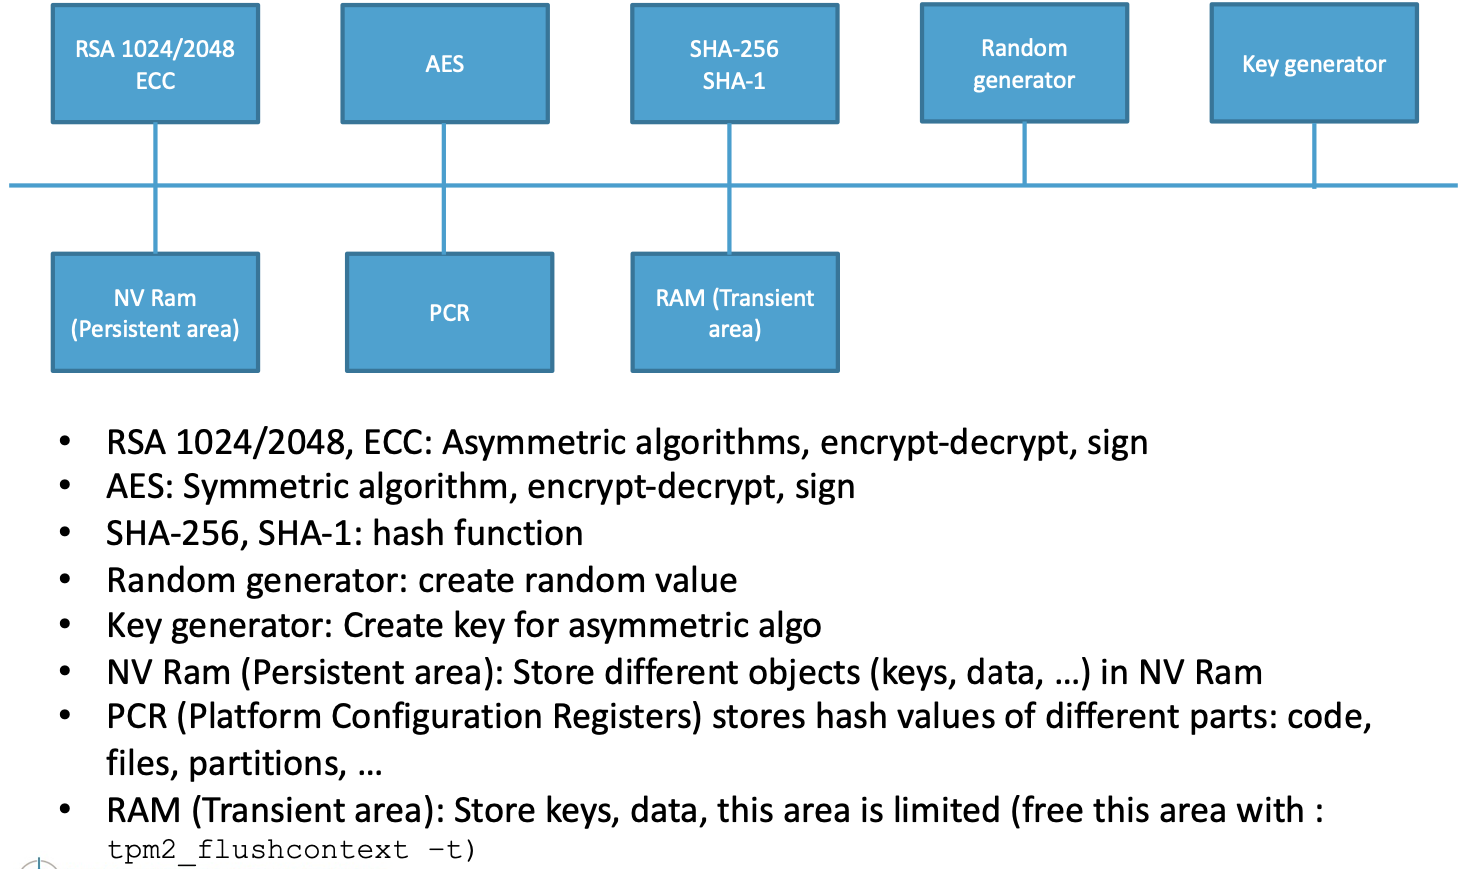
\includegraphics[width=\linewidth]{TPM.png}
\end{figure}
\begin{itemize}
    \item Discret : Circuit dédié (tamperproof)
    \item Intégré : Partie du $\mu$C qui gère le TPM
    \item Hyperviseur : fournis par personnes fiables
\end{itemize}
Peut aussi être software
% ----------
\subsubsection{Hiérarchies}
Stockage des clés
\begin{itemize}
    \item endorsement : réservé au fabricant du TPM et fixé lors de la fabrication.
    \item platform : réservé au fabricant de l'hôte et peut être modifier par l'équipementier.
    \item owner : hiérarchie dédiée à l'utilisateur primaire du TPM peut être modifié en tout temps.
    \item null : réservé aux clés éphémères (RAM s'efface à chaque redémarrage)
\end{itemize}

\subsection{Platform Configuration Registers (PCR)}
The prime use case is to provide a method to cryptographically record (measure) software state or configuration data used by a device.
\begin{figure}[H]
    \centering
    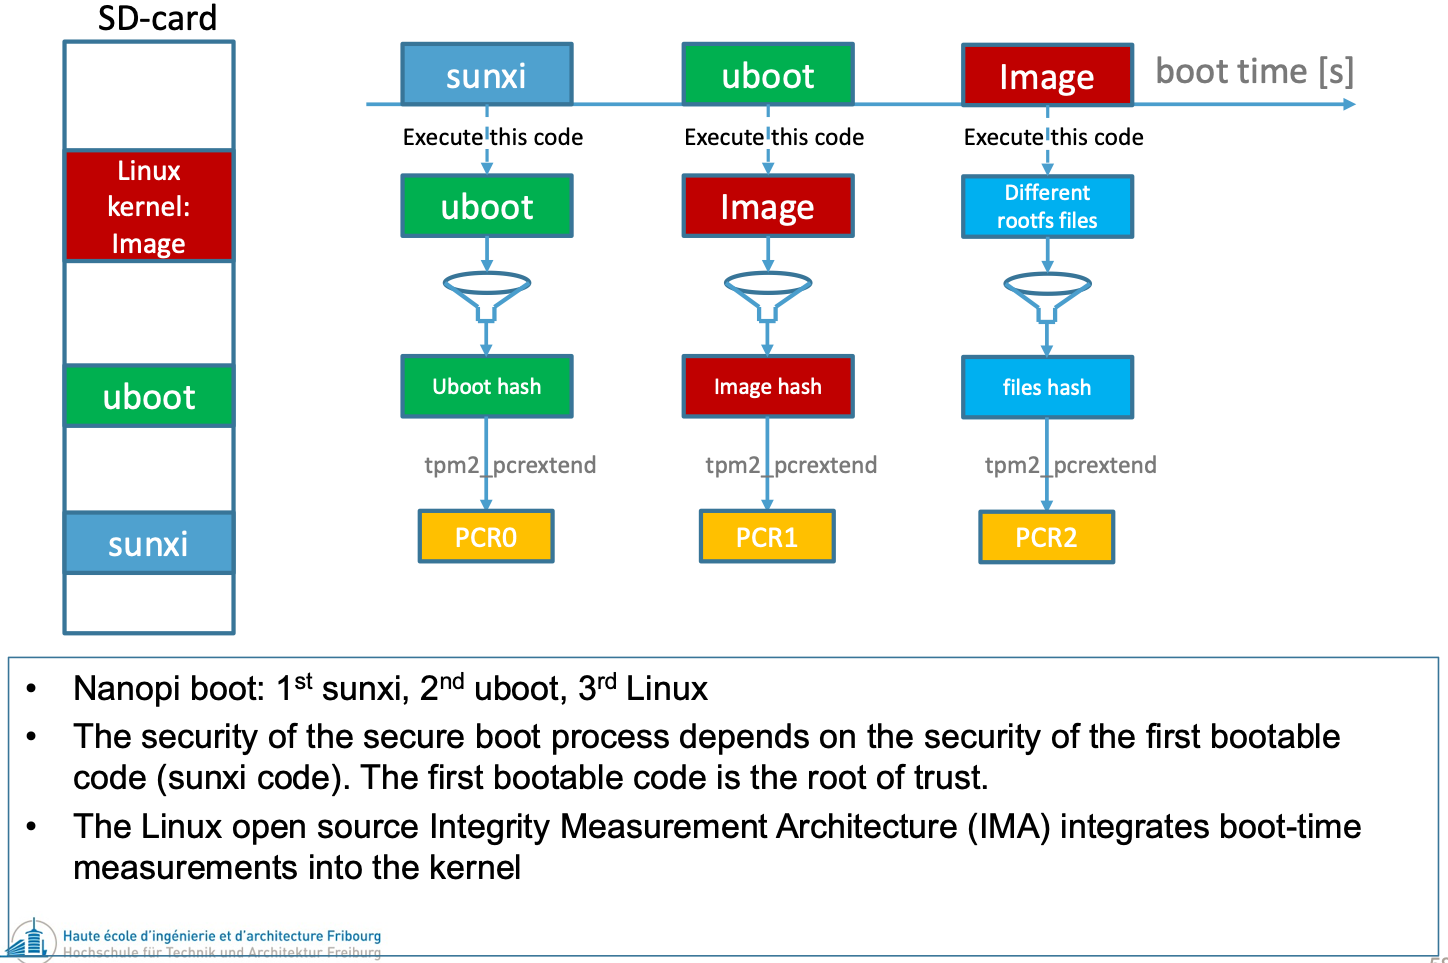
\includegraphics[width=\linewidth]{PCR.png}
\end{figure}